% following this guide 
% https://www.overleaf.com/learn/latex/How_to_Write_a_Thesis_in_LaTeX_(Part_1):_Basic_Structure

\documentclass[12pt]{book} 
\usepackage{biblatex} 
\usepackage{graphicx} % for images
\usepackage{amsmath} %for big math definitions, enables \[  \]
\usepackage{amssymb} %for common sets as real, complex, etc
\usepackage{graphicx} %for insert images
\usepackage{multicol} %for multicolumns
\usepackage{cancel} %to cancel math terms
\usepackage{float} % to use the H param in tables and fix his position
\usepackage{hyperref} % to make listofcontent clickable
\usepackage{tcolorbox} % to put te inside box

%%%%%%%%%%%%%%%%%%%%%%% list of packages to remove before release
\usepackage[figcolor=white]{todonotes}
%\todo[inline]{A todonote placed in the text}
%%%%%%%%%%%%%%%%%%%%%%%

\addbibresource{bib/biblatex.bib}
\graphicspath{ {./images/} }
\restylefloat{table} % allow the tables to use the H param
\hypersetup{
    colorlinks,
    citecolor=black,
    filecolor=black,
    linkcolor=black,
    urlcolor=black
}

\addbibresource{bib/biblatex.bib}

\begin{document}

\begin{titlepage}
    \vspace*{\stretch{1.0}}
    \begin{center}
       \Large\textbf{Statistics for Data Science}\\
       \large\textit{Ricardo Hortelano}\\
       \textit{2019}\\
       \vspace*{3\baselineskip}
       \textit{Release:}\\
       \textit{\input{version}}
    \end{center}
    \vspace*{\stretch{2.0}}
 \end{titlepage}

%%%%%%%%%%%%%%%%%%%%%% to remove before release
\listoftodos
%%%%%%%%%%%%%%%%%%%%%%
\tableofcontents

\chapter*{Preface}
\input{chapters/preface}

\chapter*{Introduction}
\todo[inline]{Write all this}
Who am I?\\
Why this book?\\
What is maths?\\
How to read?\\
How to reference it?\\
How to collaborate?


\chapter{Linear Algebra}
This chapter will focus on the very basis of mathematical knowledge and linear algebra, but builded from the very beginning.

\section{Number Sets}
\begin{itemize}
    \item Natural $\mathbb{N} = \{1, 2, 3, \dots\}$
    \item Integer $\mathbb{Z} = \{\dots, -2, -1, 0, 1, 2, \dots\}$
    \item Rational $\mathbb{Q} = \{r | r= \frac{m}{n},$ where $m,n \in \mathbb{Z}, n \neq 0\}$
    \item Irrational $\mathbb{P} = \mathbb{R} \setminus \mathbb{Q} = \{\pi, \sqrt{2}, e, \dots \}$
    \item Real $\mathbb{R} = \mathbb{P} \cup \mathbb{Q}$
    \item Complex $\mathbb{C} = \{ z = a +bi, $ where $a,b\in \mathbb{R}, i^2=-1\}$
\end{itemize}

\section{Fundamental theorem of Algebra}
Any n$^{th}$ degree polynomial, such as,
\[ r(x) = x^n + \alpha_1 x^{n-1} + \alpha_2 x^{n-2} + \dots + \alpha_{n-1}x + \alpha_n \]
has $n$ roots in $\mathbb{C}$ allowing multiplicity. Where
\begin{itemize}
    \item A root is a value such as $r(x)=0$
    \item Multiplicity means that a root can be repeat. ex: A root repeated two times is called a root with multiplicity of two.
\end{itemize} 

We can use those roots to factorize a polynomial. For example, for a polynomial of grade two we can use the formula
$\frac{-b \pm \sqrt{b^2 - 4ac}}{2a}$
\[ r(x) = ax^2 + bx + c \Leftrightarrow r(x) = a(x-x_+)(x-x_-) \]

There is also a formula for cubic polynomials (grade three)\\

For polynomials of greather grade, it can be used the Ruffini's Rule\\
TODO

\section{Linear Equations}


\chapter{Probability}
This chapter will focus on the main probabilistic knowledge necessary to have a strong mathematical base. One of the key thing to know about
probabilities is that all the theory is builded from the set theory. Because of that the very first points to take into account will be the
fundamental set aspects. After that the chapter will go inside into the probabilistic theory.

\section{Set Theory}
Informally, a set can be defined as a collection of objects. The formally definition of what it's a set vary depending of the axiomatic definition
of choice. Because set theory is not into the aim of this book and because sets can be studied intuitively, we are going to refer to it in his more 
fundamental form. Venn diagrams can be used to understand graphically most of the properties of sets.

\subsection{Notation}
If an object $o$ is an element of a set $A$, then we can write $o \in A$. A set and his elements can be denoted by
\begin{center}
    $A = \{o_1, o_2, \dots , o_n\}$ where $n$ can be \textit{finite} or \textit{infinite}
\end{center}
If all elements of a set $B$ are also member of a set $A$ then we can say that $B$ is a subset of $A$ and it's denoted by $B \subset A$ or $B \subseteq A$ 
if $A$ and $B$ has exactly the same elements.\\
Sometimes a especial set $U$ is used to refer the set that contains all possible objects.

\subsection{Binary Operations}
Set theory defines a group of operations that can be performed between two sets. Some of them are:
\begin{itemize}
    \item \textbf{Union} of $A$ and $B$, denoted $A \cup B$, is the set of all objects that are a member of $A$, or $B$, or both.
    \item \textbf{Intersection} of $A$ and $B$, denoted $A \cap B$, is the set of all objects that are members of both $A$ and $B$.
    \item \textbf{Complement} of $A$ refers to elements not contained in $A$. Denoted $\overline{A}$ or $A^c$
    \item \textbf{Difference} of $A$ and $B$, denoted $A \setminus B$, is the set of all members of $A$ that are not members of $B$
    \item \textbf{Power} of $A$, denoted $\mathcal{P}(A)$, is the set whose members are all of the possible subsets of $A$. 
\end{itemize}

\subsection{Properties}
Derived from above there is some general properties called the \textbf{fundamental properties of set algebra}. These properties 
are essential to understand the set theory. In fact, if the set theory is completely understand, these properties are automatically 
assimilated. Thus it's not necessary to memorize it. 
\begin{itemize}
   \item Commutative: 
   \begin{itemize}
        \item[] $A \cup B = B \cup A$
        \item[] $A \cap B = B \cap A$
   \end{itemize}
   \item Associative: 
   \begin{itemize}
        \item[] $(A \cup B) \cup C = A \cup (B \cup C)$
        \item[] $(A \cap B) \cap C = A \cap (B \cap C)$
   \end{itemize}
   \item Distributive:
   \begin{itemize}
        \item[] Union with Intersection: $(A \cap B)\cup C = (A\cup C) \cap (B \cup C) $
        \item[] Intersection with Union: $(A \cup B)\cap C = (A\cap C) \cup (B \cup C) $
   \end{itemize}   
   \item Neutral Element: $A \cup \emptyset = A = A \cap S$
   \item Complementation: $A \cup \overline{A} = S$ and $A\cap \overline{A} = \emptyset$
   \item Idempotence: $A \cup A = A$ and $A \cap A = A$
   \item Abosortion: $A \cup S = S$ and $A \cap \emptyset = \emptyset$
   \item Simplication: $A \cap (A \cup B) = A = A \cup (A \cap B)$
\end{itemize}

\textbf{De Morgan's laws}
\begin{itemize}
   \item $\overline{A \cup B} = \overline{A} \cap \overline{B}$
   \item $\overline{A \cap B} = \overline{A} \cup \overline{B}$
\end{itemize}

\section{Combinatory}
Also know as expertise in counting

\subsection{Rule of Product}
If there are $\alpha$ ways of doing something and $\beta$ ways of doing another thing, then there are $\alpha\beta$ ways of performing both actions.

\subsection{k-permutations}
\textbf{k-permutations of n elements:}\\
The number of \textbf{ordered sequences} with $1\leq k \leq n$ that can be formed of $n$ elements is,
\[ n(n-1)(n-2)\dots(n-k+1) = \frac{n!}{(n-k)!} \]

\subsection{k-combinations}
\textbf{k-combinations of n objects:}\\
The number of \textbf{unordered sequences} within a set with $1\leq k \leq n$ that can be formed of $n$ elements is,
\[ \binom{n}{k} = \frac{n!}{k!(n-k)!} \]

\subsection{Partitions}
$r$ groups containing $n_i$ objects each,
\[ \binom{n}{n_1,n_2\dots,n_r} = \frac{n!}{n_1!n_2!\dots n_r!} \]

\section{Random Experiments}
 A experiment is deterministic when knowing the state of the set of variables involved in the experiment the outcome is always the same.
 Conversely a experiment is random when knowing the state (or when we ignore some of these states) of the set of variables involved in
 the experiment the outcome differs. \\
 
 In other terms, \textbf{an experiment is random} if although it is repeated in the same manner every time, can result in different outcomes. 
 Thus, the fixed outcome of a random experiment is impossible to predict in advance although the number of individual possibles outcomes is known in 
 advance.
 The probability theory study the random experiments.\\

 The notation of some elements involved in a random experiment are the followings:
 \begin{itemize}
     \item \textbf{Sample Space}, is the set of all possible outcomes of the random experiment. It's denoted by $S$ or $\Omega$
     \item \textbf{Individual Outcomes}, are the type of possible outcomes of a random experiment. It's denoted by $\omega$
     \item \textbf{Event}, is a subset of $S$. Usually denoted by capital letters starting by $A$, $B$, $C$, etc. 
        Sometimes denoted by $\mathcal{F}$ for his general form. 
     \item \textbf{Null Event}, is a special event that never occurs. Denoted by $\emptyset$
     \item \textbf{Frequency} of $\omega$ is the number of times the individual outcome $\omega$ occurs in a random experiment.
     \item \textbf{Relative Frequency} of $\omega$ is the ratio between the frequency of $\omega$ and the total number of outcomes of a random experiment.
 \end{itemize}

 Once the experiment has been performed, it is said that $A$ “happened” if the outcome of the experiment ( $\omega$ ) belongs to $A$. 

 \subsection{Events Operations}
If the logical meaning from the set operations is taken and restricted to a probabilistic perspective, then a new meaning for these operations can be defined
in this new scope. Thus:
\begin{itemize}
    \item \textbf{Union} $A \cup B$ (Grammatically $A$ or $B$), occurs when either of the two events (or both of them simultaneously) do occur.
    \item \textbf{Intersection} $A \cap B$ (Grammatically $A$ and $B$), occurs when both of them do simultaneously occur.
    \item \textbf{Complementary} $\overline{A}$ (Grammatically not $A$), occurs when the event does not occur.
    \item \textbf{Difference} $A \setminus B$ (Grammatically $A$ and not $B$), occurs when the first event does occurs, but the second does not. 
                Note that $A \setminus B = A \cap \overline{B}$
\end{itemize}

\subsection{Formal Definitions}
From an formal perspective, the concept of probability has been defined multiples times. Here they are collected the fundamental ones that tries
to formalize the abstract concepts of what it's usually understand as probability and his parts.

\subsubsection{$\sigma$-algebra}
A $\sigma$-algebra (sigma-algebra) $\mathcal{A}$ over a set $\Omega$ is a family (collection) of subsets (with elements $E_1, E_2, \dots$) of $\Omega$ that satisfies:
\begin{itemize}
    \item $\emptyset \in \mathcal{A}$
    \item If $E \in \mathcal{A}$ then $\overline{E} \in \mathcal{A}$
    \item If $E_1, E_2, \dots \in \mathcal{A}$ then $\cup_{n=1}^{\infty}E_i \in \mathcal{A}$ 
\end{itemize} 

\subsubsection{$\sigma$-algebra discrete} 
The discrete $\sigma$-algebra of $\Omega$ is the power set of $\Omega$ ($\mathcal{P}(\Omega)=\{E : E \subset \Omega\}$), that is, the collection
of all subsets of $\Omega$.\\

\textbf{For example,} given a random experiment that toss one coin,
\begin{itemize}
    \item[] $H$: The coin shows head.
    \item[] $T$: The coin shows tail. 
    \item[] $S = \{H, T\},\;\;\; \mathcal{P}(S)=\{\emptyset, \{H\}, \{T\}, S\}$
\end{itemize}

\subsubsection{Measurable Space}
The pair $(\Omega, \mathcal{A})$ is a measurable space if $\mathcal{A}$ is a $\sigma$-algebra over $\Omega$

\subsubsection{Frequentist Definition}
The probability of an event $A$ is the limit of the relative frequency of that event when the number of repetitions of the experiment tends to infinity.
If the experiment is repeated $n$ times, and $n_A$ is the number of repetitions in which $A$ happens, then the probability of $A$ is
\[ P(A) = \lim_{n \rightarrow \infty} \frac{n_A}{n} \] 

\subsubsection{LaPlace's Definition}
This definition can be used for random experiments that have a finite number of outcomes and all of them are equally likely.\\
The probability of an event $A$ is the ratio between the favorable outcomes to $A$ and the total outcomes of the experiment, thus,
\[  P(A) = \frac{\#A}{\#\Omega}  \]

This implies that, given,
\[ S = \{s_1,s_2,\dots\, s_n\},\;\;\; P(s_n)=\frac{1}{n} \]

\subsubsection{Kolmogorov Definition}
The Kolmogorov definition is the only one that does not define what is a probability function. In fact, this definition stablish three axioms that must be
satisfied by any probability function. This axioms are a fundamental part of probability theory.\\
Let the pair $(\Omega, \mathcal{A})$ be a \textit{measurable space}. In it, the probability function $P$ of some event $E$, denoted $P(E)$ is an application
over the real numbers ($P: \mathcal{A} \rightarrow \mathbb{R}$) that satisfies:

\begin{itemize}
    \item \textbf{Non Negativity}: $P(E) \geq 0, \forall E \in \mathcal{A}$
    \item \textbf{Unitarity}: $P(\Omega) = 1$
    \item \textbf{Additivity}: Any countable sequence $E_1, E_2, \dots$ of disjoint events of $\mathcal{A}$, satisfies
            \[ P(\bigcup_{n=1} E_i) = \sum_{n=1} P(E_i) \]
\end{itemize}

\subsubsection{Cox's Theorem}
Used by bayesians. TODO

\subsection{Properties}
These are the properties that apply independency of the probability definition of choice.
\begin{itemize}
    \item $P(\overline{A}) = 1 - P(A)$
    \item $P(\emptyset) = 0$
    \item If $A \subseteq B$ then $P(A) \leq P(B)$
    \item $P(A\setminus B) = P(A) - P(A \cap B)$
    \item $P(A \cup B) = P(A) + P(B) - P(A \cap B)$
    \item $P(A \cup B \cup C) = P(A \cup (B \cup C)) = P(A) + P(B) + P(C) + P(A\cap B \cap C) - P(A \cap B) - P(A \cap C) - P(B \cap C)$
\end{itemize}

\subsection{Conditional Probability}
The probability of the event $A$ occurs knowing before hand that the event $B$ has occurred is,
\[  P(A|B) = \frac{P(A\cap B)}{P(B)} \]
Note that when we have a conditional probability, it can be say that $B$ becomes the new sample space of the experiment.

\subsubsection{Properties}
The conditional probability holds all the properties of the regular probability.

\subsection{Bayes Theorem}
Given a set of events $A_1, A_2, \dots, A_n$, the probability of all of them occurring simultaneously is called \textbf{probability chain rule}, and it is
\[ P(A_1\cap A_2 \cap \dots \cap A_n) = P(A_1)P(A_2|A_1)\dots P(A_n|A_1\cap \dots \cap A_{n-1}) = \prod_{k=1}^{n}P(A_k|\bigcap_{j=1}^{k-1}A_j) \]
or alternatively, in his two events form,
\[ P(A \cap B) = P(A)P(B|A)\]

\subsubsection{Total Probability Rule}
Given $A_1,\dots,A_n$ mutually exclusive (disjoint) events whose union is the whole of the sample space (partition) and assume $P(A_i) > 0$ for every $i$ .For every 
event $B$ we have
\[ P(B) = P(A_1\cap B) + \dots + P(A_n \cap B) = \prod_{k=1}^{n}P(A_k|\bigcap_{j=1}^{k-1}A_j)\]

\subsubsection{Bayes Theorem}
Knowing of above, then we can write,
\[ P(A|B) = \frac{P(A)P(B|A)}{P(B)} =  \frac{P(A)P(B|A)}{P(A_1\cap B) + \dots + P(A_n \cap B)}\]

\subsection{Independency of two events}
Two events are independence if and only if,
\[ P(A\cap B) = P(A)P(B)\]

If $A$ and $B$ are independence, then the occurrence of $A$ does no provide any information about $B$. Formally,
\begin{center}
    If $A, B$ independ. and $P(B)>0$ then $P(A|B) = \frac{P(A\cap B)}{P(B)} = \frac{P(A)\cancel{P(B)}}{\cancel{P(B)}} = P(A)$
\end{center}

\subsubsection{Conditional Independece}
Given two events $A$ and $B$, they are conditionally independence if given $C$ and $P(C)>0$, 
\[ P(A\cap B|C) = P(A\cap C|B\cap C) \]
and
\[ P(A|B\cap C) = P(A|C)\]

TODO: Draw explanatory Venn diagram 

\section{Random Variables}
When we are dealing with random experiments, it's very common to use a number to represent a event of the sample space. It's called 
random variable.\\

A \textbf{random variable} (r.v.) is the numerical outcome of a random experiment. Formally, a random variable $X$ is a mapping
$X: \Omega \rightarrow \mathbb{R}$ TODO: Write formal definition using borel sigma-algebra

It associates each outcome of a random experiment with a real number and is measurable because the inverse image of every borelian 
set does belong to the $\sigma$-algebra of events.

\subsubsection{Support of Random Variables}
We can define the support of the random variable depending of the size of the mapped set. A r.v. is:
\begin{itemize}
    \item \textbf{Discrete} if $X(\Omega)$ is a finite or numerable set.
    \item \textbf{Continious} if $X(\Omega)$ contains an interval of $\mathbb{R}$
\end{itemize}

\subsection{Probability Mass Function}
A probability mass function (p.m.f.) match a real number $x$ with the probability that an event exactly occurs.
\[ p(x)=P(X=x)=P_X(x),\;\;\; \forall x\in \mathbb{R} \]

% \includegraphics[width=2cm, height=1cm]{random_variables_1}
\subsubsection{Properties}
TODO

\subsection{Cumulative Distribution Function}
The cumulative distribution function (c.d.f.) measures the probability that an event is not greater or equal than a real number.
\[ F(x) = P(X\leq x) = P_X((-\infty,x])),\;\;\; \forall x \in \mathbb{R} \]

\subsubsection{Properties}
\begin{itemize}
    \item $\lim_{x \rightarrow -\infty} F(X) = 0$
    \item $\lim_{x \rightarrow \infty} F(X) = 1$
    \item F is non-decreasing
    \item F is right-continious
\end{itemize}

\subsection{Mean, Variance and Standard Deviation}
\subsubsection{Mean or Expectation}
Let $X$ be a r.v. with the probability function $p(x)$, then, the \textit{expected value} of $X$ is,
\[ \mu_{X} \approx \mathbb{E}[X] = \sum_{x} x\,P(X=x) \]

if $p(x)$ is an accurate characterization of the \textit{population} frequency distribution, then,
\[ \mu_{X} = \mathbb{E}[X] \]

\textbf{Properties}
\begin{itemize}
    \item $\mathbb{E}[c] = c$, if $c$ is a constant
    \item $\mathbb{E}[aX+b]=a\mathbb{E}[X]+b$
    \item $\mathbb{E}[g(x)]=\sum_{x}g(x)P(X=x)$
    \item $\mathbb{E}[X^k] = \sum_{x} x^k P(X=x)$
    \item $\mathbb{E}[X+Y] = \mathbb{E}[X] + \mathbb{E}[Y]$
    \item $\mathbb{E}[X-Y] = \mathbb{E}[X] - \mathbb{E}[Y]$
    \item $\mathbb{E}[XY] = \mathbb{E}[X]\mathbb{E}[Y]$, if $X$ and $Y$ are independent
\end{itemize}

\subsubsection{Variance}
Let $X$ be a r.v. with mean $\mathbb{E}[X] = \mu$, probability function $p(x)$, then, the variance of $X$ is defined to be the expected value of $(X-\mu)^2$, thus,
\[ \sigma^2_X \approx V[X] = \mathbb{E}[(X-\mu)^2] = \mathbb{E}[X^2] - \mu^2 = \sum_{x}(x-\mathbb{E}[X])^2 P(X=x) \]

if $p(x)$ is an accurate characterization of the \textit{population} frequency distribution, then,
\[ \sigma^2_{X} =  V[X] \]

\textbf{Properties}
\begin{itemize}
    \item $V[X] \geq 0$
    \item $V[aX + b] = a^2V[X], \;\;\; \forall a,b \in \mathbb{R}$
    \item $V[X \pm Y] = V[X] + V[Y]$, if $X$ and $Y$ are independent.
    \item $V[X + Y] = V[X] + V[Y] + 2Cov(X,Y)$
\end{itemize}

\subsubsection{Standard Deviation}
The standard deviation of $X$, is the positive square root of $V[X]$
\[ \sigma = \sqrt{V[X]} \]


\subsection{Median and Quantiles}
\subsubsection{Median}
The median is the most central value of a distribution of a r.v. $X$, thus, the median $m$ of $X$ satisfies,
\[ P(X \leq m) \geq \frac{1}{2} \]
and
\[ P(X \leq m) \leq \frac{1}{2} \]
TODO: add a explanatory image

\subsubsection{$\alpha$-quantiles}
For $0 < \alpha < 1$ the $\alpha$-quantile of a r.v. $X$ is a number $q_\alpha$ that satisfies,
\[ P(X \leq q_\alpha) \geq \alpha \] 
and
\[ P(X \geq q_\alpha) \geq 1- \alpha \]
TODO: add a explanatory image

\subsection{Quantile Function}
For $0 < \alpha < 1$ the \textit{quantile function} of a r.v. is defined as,
\[ F^{-1}_X (\alpha) = \inf \{ x : F(x) \geq \alpha  \} \]
TODO: add a explanatory image

\subsubsection{Properties}
TODO

\section{Discrete Random Distributions}
\subsection{Bernoulli Process}
A \textbf{Bernoulli process} is random experiment in which outcome can only result in two different values. This outcomes are
commonly refered as \textit{success} and \textit{failure}. The probability of success is $0 \leq p \leq 1$ and all experiment
trials are \textit{independent}.
\[ X \sim Bernoulli(p) \]

\subsection{Binomial Distribution}
Consider a Bernoulli process with probability of success $p$ and that is carried out independently $n$ times, a Binomial random variable 
$X$ with parameters $n$ and $p$ represents the number of trials that result in success.
\[ X \sim B(n, p) \]
with
\[ P(X=x) = \binom{n}{x}p^x(1-p)^{n-x},\;\;\; x \in \{0,1,2,\dots,n\} \]
and have expectation and variance
\[ \mathbb{E}[X] = np,\;\;\; V[X] = np(1-p) \]

\textbf{Note: Be careful with the definition.} It's not the same 'number of trials' and 'number of success'.


\subsubsection{Properties}
If $X$ and $Y$ are independent, and $X \sim B(n_1, p), Y \sim B(n_2, p)$ then 
\[ X+Y \sim B(n_1+n_2, p) \]

\begin{figure}[!ht]
    \begin{minipage}{0.45\linewidth}
      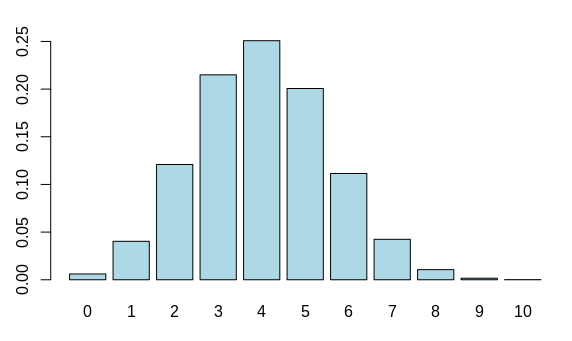
\includegraphics[width=1\linewidth]{random_distribution_binomial_1}
      \caption{Binomial p.m.f.}
    \end{minipage}
    \hfill
    \begin{minipage}{0.45\linewidth}
      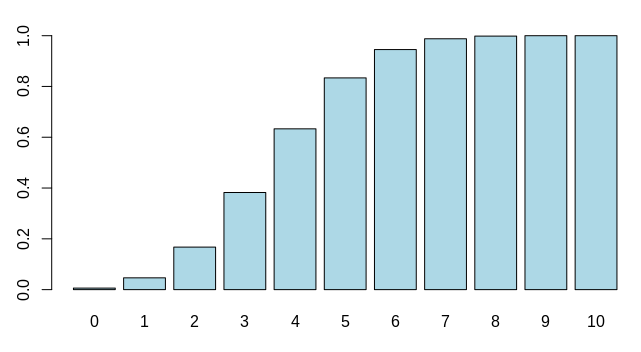
\includegraphics[width=1\linewidth]{random_distribution_binomial_2}
      \caption{Binomial c.d.f.}
    \end{minipage}
\end{figure}

\subsection{Geometric Distribution}
Consider a Bernoulli trial with probability of success $p$, the number of independent trials that result in \textit{failure} obtained before 
the first success follows a Geometric distribution with parameter $p$.
\[ X \sim \mathcal{G}(p)\]
with
\[ P(X=x) = p(1-p)^x,\;\;\; x \in \{0,1,2,\dots,n\} \]
and have expectation and variance
\[ \mathbb{E}[X] = \frac{1-p}{p},\;\;\; V[X] = \frac{1-p}{p^2} \]

\begin{figure}[!ht]
    \begin{minipage}{0.45\linewidth}
      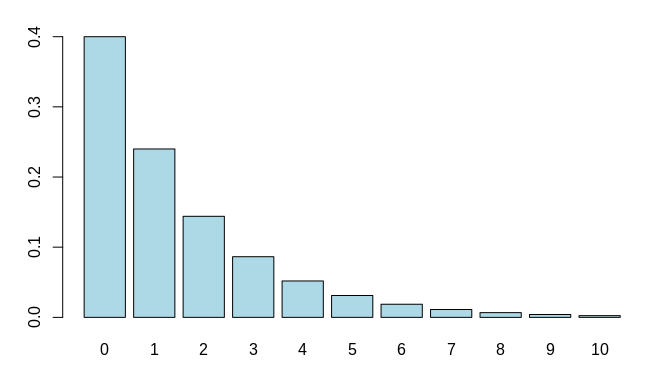
\includegraphics[width=1\linewidth]{random_distribution_geometric_1}
      \caption{Geometric p.m.f.}
    \end{minipage}
    \hfill
    \begin{minipage}{0.45\linewidth}
      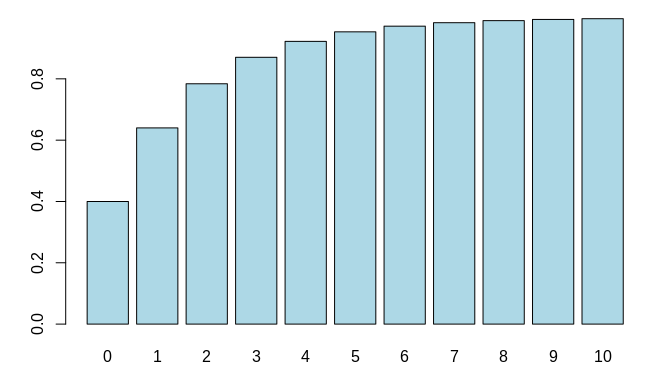
\includegraphics[width=1\linewidth]{random_distribution_geometric_2}
      \caption{Geometric c.d.f.}
    \end{minipage}
\end{figure}

\subsection{Negative Binomial Distribution}
Consider a Bernoulli trial with probability of success $p$, the number of failures (independent trials that result in failure) before the $k$-th success 
(that is, \textbf{number of trials} until $k$-success) follows a Negative Binomial distribution with parameters $k$ and $p$.
\[ X \sim NB(k,p)\]
with
\[ P(X=x) = \binom{x+k-1}{x} p^k(1-p)^x,\;\;\; x \in \{0,1,2,\dots,n\} \]
and have expectation and variance
\[ \mathbb{E}[X] = \frac{k(1-p)}{p},\;\;\; V[X] = \frac{k(1-p)}{p^2} \]

\textbf{Note: Be careful with the definition.} It's not the same 'number of trials' and 'number of success'.

\begin{figure}[!ht]
    \begin{minipage}{0.45\linewidth}
      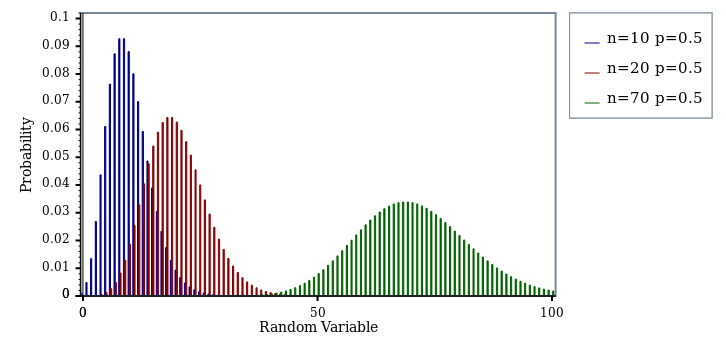
\includegraphics[width=1\linewidth]{random_distribution_negbinomial_1}
      \caption{Negative Bin. p.m.f.}
    \end{minipage}
    \hfill
    \begin{minipage}{0.45\linewidth}
      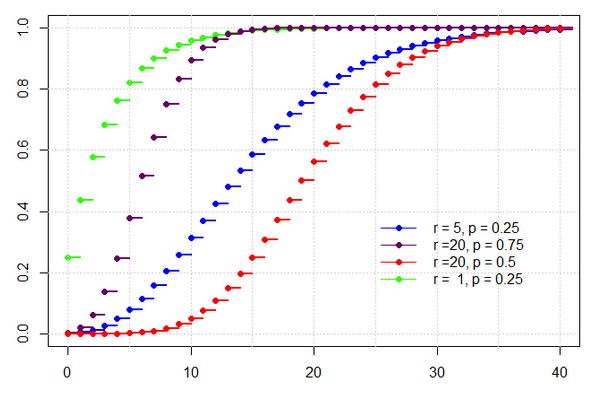
\includegraphics[width=1\linewidth]{random_distribution_negbinomial_2}
      \caption{Negative Bin. c.d.f.}
    \end{minipage}
\end{figure}

\subsection{Hypergeometric Distribution}
Consider a \textbf{finite population} with $N_1+N_2$ objects, such that $N_1$ are of type 1 and $N_2$ are of type 2. A total number of $k$
objects are selected from the population \textbf{without replacement}. The number of objects of type $N_1$ in the selection follows 
a Hypergeometric distribution with parameters $N_1, N_2$, and $k$.
\[ X \sim H(N_1,N_2,k)\]
with
\[ P(X=x) = \frac{\binom{N_1}{x}\binom{N_2}{k-x}}{\binom{N_1+N_2}{k}},\;\;\; x \in \{\max\{0,k-N_2\},\dots,\min\{k,N_1\} \} \]
and have expectation and variance
\[ \mathbb{E}[X] = \frac{kN_1}{N_1+N_2},\;\;\; V[X] = k\cdot\frac{N_1N_2}{(N_1+N_2)^2}\cdot\frac{N_1+N_2-k}{N_1+N_2-1} \]

\begin{figure}[!ht]
    \begin{center}
        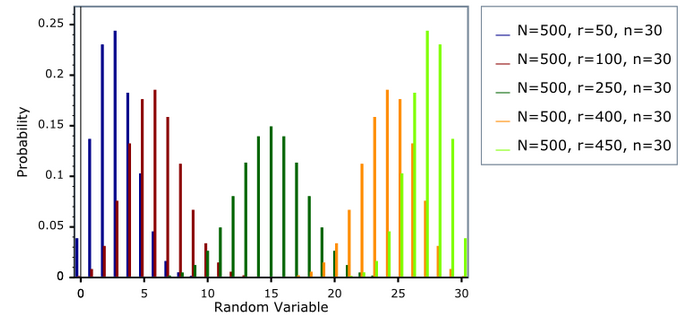
\includegraphics[width=0.4\linewidth]{random_distribution_hyperg_1}
        \caption{Hypergeometric p.m.f.}
    \end{center}
\end{figure}

\subsection{Poisson Distribution}
The number of events that occur in a region of space (or time) independently one from the others and at a constant rate $\lambda >0$ 
follows a Poisson distribution with parameter $\lambda$.
\[ X \sim \mathcal{P}(\lambda)\]
with
\[ P(X=x) = e^{-\lambda}\frac{\lambda^x}{x!},\;\;\; x \in \{0,1,2,\dots,n\} \]
and have expectation and variance
\[ \mathbb{E}[X] = \lambda,\;\;\; V[X] = \lambda \]

\subsubsection{Properties}
If $X$ and $Y$ are independent, and $X \sim \mathcal{P}(\lambda_1), Y \sim \mathcal{P}(\lambda_2)$ then 
\[ X+Y \sim \mathcal{P}(\lambda_1+\lambda_2) \]

\begin{figure}[!ht]
    \begin{minipage}{0.45\linewidth}
      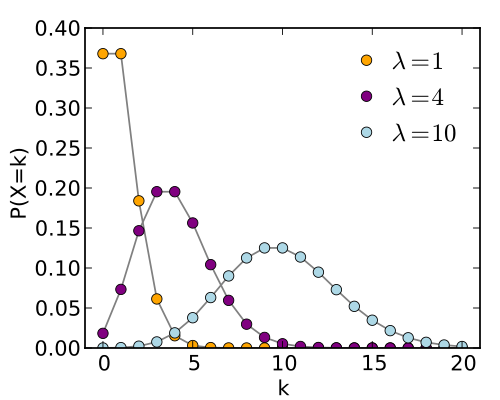
\includegraphics[width=1\linewidth]{random_distribution_poisson_1}
      \caption{Poisson p.m.f.}
    \end{minipage}
    \hfill
    \begin{minipage}{0.45\linewidth}
      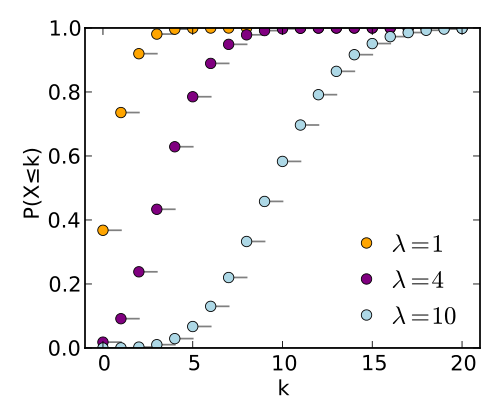
\includegraphics[width=1\linewidth]{random_distribution_poisson_2}
      \caption{Poisson c.d.f.}
    \end{minipage}
\end{figure}

\subsection{Multi Bernoulli Distribution}
TODO


\subsection{Zero Inflated Poisson Distribution}
TODO


\chapter{Statistical Inference}
This chapter will focus in the procedures to analyze a phenomena of which some information is unknown. Until now,
we had analyzed problems and experiments in which the whole structure of the problem is known before. But, what
happen when we couldn't know the probabilities related with all events? There is any approach to overcome this?
Someone could just think, "Well, lets perform the experiment $n$ times and let's see what happen."\\

This approach is the one we are going to follow in this chapter, and in it, it's analyzed the problems and benefits
of performing such approach. The only prior we have to take in to account is that 
\textbf{all random phenomena follows an underlying probability function}. With this in mind. Let's start defining in 
a formal way "perform the experiment $n$ times"

\subsection{Parametric Family of Distributions}
Let $F$ be a p.d.f. with parameter $\theta$\\

Usually, for some random experiments, the trials could give us some information about the shape of the underlying
probability function $F$ of the experiment. In practice, $F$ is not exactly know, but we know that his parameter 
$\theta$ model his shape. So, we can know that $F$ belongs to a set or \textit{parametric family of distributions}
$\{F(\;\cdot\;;\theta)\; |\; \theta \in \Theta\}$.\\

Because our objective is to know more about the real $F$ we need to perform some procedures in order to \textit{infer}
the real value of $\theta$. If we achieve to infer the real value, or at least, an approximately one, then we could find,
a good approximation of $F$ inside his family of distributions. In order to extract this information about $F$ we need
to perform independent realizations of the experiment related with $F$. With this extracted knowledge we could perform
inference over $F$ or his parameter $\theta$.\\

The fact that we perform independent repetitions of the experiment means that, for each repetition of the experiment, 
we have an associated r.v. with the same distribution $F$. This is called, \textit{simple random sample}.

\subsection{Types of estimation (Inference)}
TODO
\begin{itemize}
    \item Model Based (exact, approximated)
    \item Sampling Based
    \item Bayesian Based
\end{itemize}

\subsection{Random Sample}
A \textit{simple random sample} of a r.v. $X$ with distribution $F$ is a collection of r.v. $(X_1, X_2,\dots,X_n)$ that are 
\textbf{independent and identically distributed (i.i.d.)} and all of them follows the same distribution $F$\\

Because the random variables are independent, the c.d.f. of the sample is,
\[ F_X(x_1,x_2,\dots,x_n) = F(X_1)F(x_2)\dots F(x_n) \]

\subsection{Statistic}
A statistic $T$ is any measurable function $T: (\mathbb{R}^n,\mathcal{B}^n) \rightarrow (\mathbb{R}^k,\mathcal{B}^k)$, where $k$ 
is the dimension of the statistic. For example:
\begin{itemize}
    \item $T_1(X_1,X_2,\dots,X_n) = \frac{1}{n}\sum_{i=1}^{n}X_i \triangleq \bar{X}_n$, this is called \textbf{Sample Mean}
    \item $T_1(X_1,X_2,\dots,X_n) = \frac{1}{n-1}\sum_{i=1}^{n} (X_i-\bar{X})^2 \triangleq S'^2_n$, this is called \textbf{Sample Variance}
    \item $T_1(X_1,X_2,\dots,X_n) = \min \{ X_1,\dots,X_n \} \triangleq X_{(1)}$
    \item $T_1(X_1,X_2,\dots,X_n) = \max \{ X_1,\dots,X_n \} \triangleq X_{(n)}$
    \item $T_1(X_1,X_2,\dots,X_n) = \sum_{i=1}^{n} \log{X_i}$
    \item $T_1(X_1,X_2,\dots,X_n) = (X_{(1)}, X_{(n)})$
\end{itemize} 
All these statistics have dimension $k=1$ except the last with $k=2$. The distribution induced by the statistic $T$ is called the 
\textit{sampling distribution} of $T$, since it depends on the distribution of the sample.

\subsection{Estimators or Point Estimators}
An estimator is an statistic that tries to estimate the value of a parameter $\theta$ that belongs to the distribution of the variable
$X$. Thus,\\

Let $X \sim F(\cdot\;;\;\theta)$ where $\theta$ is a parameter vector with possibles values in the \textit{parameter space} $\Theta$.
An estimator $\hat{\theta}_n$ of $\theta$ is a statistic $\hat{\theta}_n(X_1,\dots,X_n)$ with values also in $\Theta$ 

To clarify with a example, in the real world many r.v. follows a normal distribution with mean $\mu \in \mathbb{R}$ and variance 
$\sigma^2 \in \mathbb{R}^+$ that are unknown. Because of this, it's usually assumed that the distribution of a r.v. belong to a 
normal family of distributions $\{\mathcal{N}(\mu,\sigma^2):\mu\in\mathbb{R},\sigma^2\in \mathbb{R^+} \}$. Knowing this, it is said 
that the \textbf{sample mean} $\bar{X}$ and the \textbf{sample variance} $S^2$ are good estimators of the distribution mean $\mu$ 
and distribution variance $\sigma^2$.

\begin{table}[H]
    \centering
    \begin{tabular}{ll}
    Population Parameter    & Sample Estimator                          \\
    $p = P(X=1)$            & $\hat{p}_n = \frac{1}{n}\sum_{i=1}^n X_i$ \\
    $\mu = \mathbb{E}[X]$   & $\bar{X}_n = \frac{1}{n}\sum_{i=1}^n X_i$ \\
    $\sigma^2 = V[X]$       & $S'^2_n = \frac{1}{n-1}\sum_{i=1}^{n} (X_i-\bar{X})^2 $
    \end{tabular}
\end{table}

\subsection{Biased and Unbiased Estimator}
TODO

\section{Exact inference under Normal Distributions}
\textbf{Sampling distributions in Normal Populations}\\
The sample mean $\bar{X}$ and sample variance $S^2$ estimators play an important role in statistical inference, since both are “good” estimators
of $\mu$ and $\sigma^2$, respectively. As a consequence, it is important to obtain their sampling distributions in order to know their random behaviors. 
We will do so under the assumption of normal populations.

\subsection{Expected value and Variance of the sample mean}
Let $\bar{X}_n = \frac{1}{n}\sum_{i=1}^n X_i$ be the sample mean. Then, it holds,
\[ \mathbb{E}[\bar{X}_n] = \mu,\;\;\; V[\bar{X}_n] = \frac{\sigma^2}{n} \]

\subsection{Expected value of the sample variance}
Let $S'^2_n = \frac{1}{n-1}\sum_{i=1}^{n} (X_i-\bar{X})^2 $ be the sample variance. Then, it holds,
\[ \mathbb{E}[S'^2_n] = \sigma^2 \]

\subsection{Logarithmic Distribution Transformations}
\textbf{TODO: Review this}
If we take a constant $k$ and perform a logarithmic transformation of the sample distribution $\bar{X}_n$ with this constant. For a fixed $k$ it holds,
\[ \log(\bar{X}_n + k) \sim \mathcal{N}(\mu, \sigma^2) \]

\subsection{Sample Mean of Normal Distribution}
Let $(X_1,\dots,X_n)$ a s.s.m. of size $n$ of a r.v. $\mathcal{N}(\mu,\sigma^2)$. Then, the \textbf{sample mean} $\bar{X}_n = \frac{1}{n}\sum_{i=1}^n X_i$
satisfies,
\[ \bar{X} \sim \mathcal{N}(\mu,\frac{\sigma^2}{n}) \]

\subsection{Z statistic or Standarization}
The $Z$ statistic is obtained when the sample mean is standarizated,
\[ Z = \frac{\bar{X}_n - \mu}{\sigma / \sqrt{n}} \sim \mathcal{N}(0,1) \]

\subsection{Chi-Square Distribution}
A Chi-square distribution $\mathcal{X}_n^2$ with $n$ degrees of freedom, is the distribution that gives the sum of $n$ independent r.v. $Z_1,\dots,Z_n$ all of
them with $\mathcal{N}(0,1)$ distributions. Thus,
\[ \sum_{i=1}^n Z_i^2 \sim \mathcal{X}_n^2 \]
and it holds that $\mathcal{X}^2_n = $Gamma$(n/2,2)$

\subsection{Fisher's Theorem}
Let $(X_1,\dots,X_n)$ be a s.r.s of r.v. that follows $\mathcal{N}(\mu,\sigma^2)$. Then,
\[ \frac{(n-1)S'^2_n}{\sigma^2} = \sum_{i=1}^{n} (\frac{X_i - \hat{X}_n}{\sigma})^2 \sim \mathcal{X}_{n-1}^2 \]
and
\begin{center}
    $\hat{X}_n$ and $\mathcal{X}_n^2$ are independent
\end{center}

\subsubsection{Dregrees of freedom remark}
TODO, diapo 2.21

\subsection{Student's Distribution}
Let $X \sim \mathcal{N}(0,1)$ and $Y \sim \mathcal{X}_v^2$ be independent. The distribution of the r.v. 
\[ T = \frac{X}{\sqrt{Y/v}} \]
is a Student's $t_v$ with $v$ degrees of freedom

\subsection{T statistic}
Let $(X_1,\dots,X_n)$ a s.r.s. of a r.v. that follows a $\mathcal{N}(\mu,\sigma^2)$. Then, a $T$ statistic is,
\[ T = \frac{\bar{X_n}-\mu}{S'^2_n / \sqrt{n}} \sim t_{n-1}\]

\subsection{Snedecor's Distribution}
Let $X_1 \sim \mathcal{X}_{v_1}^2$ and $X_2 \sim \mathcal{X}_{v_2}^2$ be independent. The distribution of the r.v.
\[ F = \frac{X_1/v_1}{X_2/v_2} \]
is a Snedecor's $F$ distribution with $v_1$ degrees of freedom in the numerator, and $v_2$ degrees of freedom in the denominator. It's denoted $\mathcal{F}_{v_1,v_2}$

\subsubsection{Note:}
\[ F_{1,v} = t^2_v \]

\subsection{F statistic}
Let $(X_1,\dots,X_{n_1})$ be a s.r.s. of a $\mathcal{N}(\mu_1,\sigma^2_1)$ with sample variance $S'^2_n$. Let $(Y_1,\dots,Y_{n_2})$ be a different s.r.s. of a 
$\mathcal{N}(\mu_2,\sigma^2_2)$ with sample variance $S'^2_2$. Let the first and the second distributions be independent. Then,
\[ F = \frac{S'^2_1/\sigma^2_1}{S'^2_2/\sigma^2_2} \sim \mathcal{F}_{n_1-1,n_2-1}\]

\section{Large Sample Inference}
What happens when we can't ensure that the underlying distribution is a normal?

\subsection{Convergence in distribution}
The sequence of r.v. converges in distribution to the r.v. $X$ if,
\[ \lim_{x\rightarrow\infty}F_{X_n}(x) = F_X(x) \]
for all the points $x$ where $F_X(x)$ is continuous. This is denoted as,
\[ X_n \xrightarrow{d} X \]  

\subsection{Central Limit Theorem}
Let $X_1,\dots,X_n$ i.i.d. r.v. with expectation $\mathbb{E}[X_i] = \mu$ and variance $V[X_i]=\sigma^2 < \infty$. Then, the c.d.f. of the r.v. converges to the c.d.f 
of a $\mathcal{N}(0,1)$ as long as $n \rightarrow \infty$. This is,
\[ Z_n = \frac{\bar{X}_n - \mu}{\sigma/\sqrt{n}} \xrightarrow{d} \mathcal{N}(0,1)\]


\textbf{TODO: insert summary of CLT}














\chapter{Numerical Methods}
This chapter will focus on the methods and processes needed to choose the optimal 
solution given a mathematical model. This chapter also include the processes needed to build these models.\\

This field of study is also know as \textbf{Prescriptive Analysis} or \textbf{Operations Research}.

The schematic way to proceed in this problems is the following:
\begin{center}
    Problem Description $\rightarrow$ Model Formulation $\rightarrow$ Analysis \& Algorithms $\rightarrow$
    Computer Solution $\rightarrow$ Interpretation
\end{center}

\section{Notation}
\subsection{Elements}
The elements involved in all mathematical decision models are the following:
\begin{itemize}
    \item Decision Variables: Are the ones we want to know his optimal value. (e.g. number of products to 
    build in a period of time)
        \[ x = (x_1, x_2, \dots , x_n) \]
    \item Objective Function: Is the one that model the problem. It will be always needed to \textit{maximize} or \textit{minimize} it.
    \begin{center}
        $\text{maximize } f(x)$ or $\text{minimze } f(x)$
    \end{center}
    \item Functional Constraints (or structural constrains): Are the limitations to the objective function and is a function of all the variables.
        \[ a_{11}x_1 + a_{12}x_2 + \dots + a_{1n}x_n \leq b_1 \]
    \item Non-negativity Constraints: Are the limitations to the objective function.
        \[ g_1(x)\leq b_1,\;\; g_2(x)\geq b_2, \;\; b_3=b_3 \]
\end{itemize}

The main goal to a correct model building is to identify these elements and define it in a proper way. Contrary that the logic 
intuition could make us think, simplest models are better than complex one with lot of constraints and elaborated objective functions. \\

\textbf{All models are wrong, but some are useful} (? citation)\\

Why use this models? Because most of the times the time and memory computational complexity to resolve some problems in a brute force
or in a non analytical way is way greater than the models developed using this approach.

\subsection{Standard Form of the Model}
A problem is described in the standard form if it is described in the following way:\\
\[ \text{maximize } c_1x_1 + c_2x_2 + \dots + c_nx_n\]
Subject to the restrictions
\begin{gather*}
    a_{11}x_1 + a_{12}x_2 + \dots + a_{1n}x_n \leq b_1 \\
    a_{21}x_1 + a_{22}x_2 + \dots + a_{2n}x_n \leq b_2 \\
    \dots\\
    a_{m1}x_1 + a_{m2}x_2 + \dots + a_{mn}x_n \leq b_m
\end{gather*}
and
\[ x_1 \geq 0,\;\;\; x_2 \geq 0,\;\;\; \dots\;\;\; x_n \geq 0 \]

\subsection{Other Forms}
\begin{itemize}
    \item Minimizing rather than maximizing the objective function.
    \[ \text{minimize } c_1x_1 + c_2x_2 + \dots + c_nx_n\]
    \item Functional constrains with a greather-or-equal inequality
    \[ a_{i1}x_1 + a_{i2}x_2 + \dots + a_{in}x_n \geq b_i \]
    \item Functional constrains in equation form
    \[ a_{i1}x_1 + a_{i2}x_2 + \dots + a_{in}x_n = b_i \]
    \item Deleting the non-negativity constrains
    \[ x_j \text{is unrestricted in sign for some values of } j \]
\end{itemize}

\subsection{Terminology for solutions of the model}
\begin{itemize}
    \item \textbf{Feasible solution} is a solution that satisfies all the constrains. It is possible for a problem to have no feasible solutions.
    \item \textbf{Infeasible solution} is a solution with at least one constrains unsatisfied.
    \item \textbf{Feasible region} is the set of possibles solutions of the model. It's always a convex polytope. This polytope is defined by the intersection of the problem constraints
    \item \textbf{Optimal solution} of the problem. Is whose that \textit{maximize} or \textit{minimize} the objective function inside the feasible region. 
    Usually, this optimal solution is find computationally. It is possible for a problem to have multiples optimal solutions, also is possible to do not have them.
    \item A \textbf{Corner-point feasible (CPF)} solution is a solution that lies at a corner of the feasible region.
\end{itemize}

\subsubsection{Realtionship between optimal solutions and CPF solutions}
Consider any linear pro-gramming problem with feasible solutions and a bounded feasible region. The problem
must possess CPF solutions and at least one optimal solution. Furthermore, the best CPF
solution must be an optimal solution. Thus, if a problem has exactly one optimal solution,
it must be a CPF solution. If the problem has multiple optimal solutions, at least two must
be CPF solutions.


\section{Linear Optimization (LO) Models}
Most important type of decision optimization models. Is the foundation to understand the complex ones. Also is one of the most widely
applied models because of his simplicity.\\

\subsubsection{Limitations}
\begin{itemize}
    \item Decision variables needs to be continuous. 
        \[x = (x_1, x_2, \dots , x_n) \in \mathbb{R}\]
    \item Objective function needs to be linear in $x$. Called \textit{}.
        \[ f(x_1,x_2, \dots, x_n) = c_1x_1 + c_2x_2 + \dots + c_nx_n \]
    \item Constraints needs to be linear in $x$
        \begin{gather*}
            a_{11}x_1 + a_{12}x_2 + \dots + a_{1n}x_n \leq b_1 \\
            a_{21}x_1 + a_{22}x_2 + \dots + a_{2n}x_n \leq b_2 \\
            \dots\\
            a_{m1}x_1 + a_{m2}x_2 + \dots + a_{mn}x_n \leq b_m
        \end{gather*}
    \item Decision Variables needs to be non-negative
        \[ x_1 \geq 0,\;\;\; x_2 \geq 0,\;\;\; \dots\;\;\; x_n \geq 0 \]
\end{itemize}

An equation in a form called \textbf{Slope-intercept form} is the one in the form $x_n = ax_i + bZ,\;\; \forall a,b \in \mathbb{R}$ and demonstrate that the slope of the line is $a$. This means that an increase
of one value in $x_n$ implies an increment of $a$ in $x_i$. Whereas, the intercept of the line with the $x_n$ axis is $bZ$.\\

\subsubsection{Assumptions of a LO problem}
\begin{itemize}
    \item Proportionally, realted with linearity of the objective functions and constrains.
    \item Additivity, Every function is the sum of the individual contributions of the respectives activities.
    \item Divisibility, decision variables are in $\mathbb{R}$
    \item Certainty, the value assigned to each parameter is assumed to be a known constant. This allow us to perform sensitivity analysis.
\end{itemize}

\subsection{Duality}
Every linear programming problem has associated with it another linear programming
problem called the \textbf{dual}.\\

Wikipedia\\
The duality principle is the principle that optimization problems may be viewed from either of two perspectives, the \textbf{primal problem} or the \textbf{dual problem}. 
The solution to the dual problem provides a lower bound to the solution of the primal (minimization) problem. However in general the optimal values of 
the primal and dual problems need not be equal. Their difference is called the duality gap. For convex optimization problems, the duality gap is zero under 
a constraint qualification condition. \\

These conditions are:
\begin{itemize}
    \item Non-negative variables
    \[x = (x_1^+, x_2^+, \dots , x_n^+) \in \mathbb{R}\]
    \item The objective functions need to be maximize
    \[ \text{maximize } c_1x_1 + c_2x_2 + \dots + c_nx_n\]
    \item All constrains must be equality (non inecuations)
    \[ a_{m1}x_1 + a_{m2}x_2 + \dots + a_{mn}x_n = b_m \]
    \item The right-hand side values must be non-negatives
    \[ b_m > 0,\;\; \forall m \in \{1,2,\dots,m\} \]
\end{itemize}

If some of this conditions are not satisfied, we can convert the equations to make it satisfied.\\
\textbf{For constrains that are non-equality}\\
Given, $x_1 \leq 4$ we can convert it to a new variable. Just,
\[ x_1 \leq 4 \equiv  x_3 = 4 - x_1\]
This new variable $x_3$ is called \textbf{slack or surplus variable} depending of what is doing. So for a problem,
\setlength{\columnseprule}{1pt}
\begin{multicols}{2}
    Original Problem \begin{multline*} 
        \text{maximize } Z = 3x_1 + 5x_2 \\
        \text{subject to }\\
        x_1 \leq 4\\
        2x_2 \leq 12
    \end{multline*}

    Augmented Problem \begin{multline*}
        \text{maximize } Z = 3x_1 + 5x_2 \\
        \text{subject to }\\
        x_1 + x_3 = 4\\
        2x_2 + x_4 = 12
    \end{multline*}
\end{multicols}
\textbf{For variables with unrestricted sign}\\
TODO

\subsubsection{Formulation}
\setlength{\columnseprule}{1pt}
\begin{multicols}{2}
    Primal Problem \begin{multline*} 
        \text{maximize } Z = \sum_{j=1}^n c_jx_j \\
        \text{subject to }\\
        \sum_{j=1}^n a_{ij}x_j \leq b_i, \;\;\; \forall i \in \{1,2,\dots,m\}\\
        \text{and}\\
        x_j \geq 0, \;\;\; \forall j \in \{1,2,\dots,n\}
    \end{multline*}

    Dual Problem \begin{multline*}
        \text{minimize } W = \sum_{i=1}^m b_iy_i \\
        \text{subject to }\\
        \sum_{i=1}^m a_{ij}y_i \leq c_j, \;\;\; \forall j \in \{1,2,\dots,m\}\\
        \text{and}\\
        y_i \geq 0, \;\;\; \forall i \in \{1,2,\dots,n\}
    \end{multline*}
\end{multicols}

\subsubsection{Properties}
\begin{itemize}
    \item \textbf{Weak duality}: If $x$ is a feasible solution for the (P) and $y$ is a feasible solution for (D), then
    \[ cx \leq yb \]
    \item \textbf{Strong duality}: If $x^*$ is an optimal solution for (P) and $y^*$ is an optimal solution for (D), then,
    \[ cx^* = y^*b \]
\end{itemize}
Thus, these two properties imply that $cx < yb$ for feasible solutions if one or both of them
are not optimal for their respective problems, whereas equality holds when both are optimal.

\begin{itemize}
    \item \textbf{Symmetry property}: For any primal problem and its dual problem, all relationships between them must be 
    symmetric because the dual of this dual problem is this primal problem.
\end{itemize}

\subsubsection{Relation between primal and dual problem}
The following are the only possible relationships between the two problems.
\begin{enumerate}
     \item If one problem has feasible solutions and a bounded objective function (and
     so has an optimal solution), then so does the other problem, so both the weak
     and strong duality properties are applicable.
     \item If one problem has feasible solutions and an unbounded objective function
     (and so no optimal solution), then the other problem has no feasible solutions.
     \item If one problem has no feasible solutions, then the other problem has either no
     feasible solutions or an unbounded objective function.
\end{enumerate}

\subsubsection{Complementary Basic Solutions}
Because the problem (D) is also a LO problem, it also has a corner point solution. Ussing the augmented form of the problem 
we can express these corner-point solution as a basic solution. Because the functional constrains have $\geq$, this solution
is obtained by subtracting the surplus (rather than adding the slack) from the Left-HS of each constraint $j$. Thus,
\[ z_j - c_j = \sum_{i=1}^m a_{ij}y_i - c_j,\;\; \forall j \in \{1,2,\dots,n\} \]
So $z_j-c_j$ is the \textbf{}{surplus variable} for constraint $j$ (or its slack variable if
the constraint is multiplied through by -1). \\

One of the important relationships between the primal and dual problems is a direct cor-
respondence between their basic solutions.
\begin{itemize}
    \item \textbf{Complementary basic solutions property}: Each basic solution in the primal
    problem has a \textbf{complementary basic solution} in the dual problem, where their
    respective objective function values (Z and W) are equal.
    \item \textbf{Complementary slackness property}: CHECK THIS and addapt to the defition given here
    \[ (\sum_{i=1}^m a_{ij}\pi_i - r_j) \bar{x}_j = 0, \;\; \forall j \in \{ 1,2,\dots,n \} \]
\end{itemize}


\subsection{Sensitivity Analysis}
Once we already have the optimal solution for a LO problem, it would be important to analyze if slight changes in the constraints or the objective function
affects the optimal solution or it remains the same. Specifically, we would want to analyse and find the \textbf{parameter bounds} of the optimal solution.
We are going to analyze two types of changes:
\begin{enumerate}
    \item Changes in objective coefficients
    \item Changes in the right-hand side of the constraints    
\end{enumerate}

\subsubsection{Changes in objective coefficients}
\textbf{Simplified example.}\\
Given an objective function (o.f.),
\[ \text{maximize } z(x_1, x_2) = 5x_1 + 4x_2 \]
Subject to
\[ \text{M1: } 6x_1 + 4x_2 \leq 24 \]
\[\text{M2: } x_1 + 2x_2 \leq 6 \]
with optimal solution in $x^* = (3, 3/2)$, we can perform the sensitivity analysis if the changes in the o.f. are expressed as,
\[ \text{maximize } \hat{z}(x_1, x_2) = (5+\Delta r_1)x_1 + (4 + \Delta r_2)x_2 \]

\textbf{Solution:}\\
We know that $x^* = (3, 3/2)$ for $(\Delta r_1, \Delta r2) = 0$, but, for which increments of $(\Delta r_1, \Delta r2)$ is optimal $x^*$?
$x^*$ is optimal only and only if
\begin{center}
    slope of M1 constraint $\leq$ slope of $\hat{z} \leq$ slope of M2 constraint
\end{center} 
\[ -\frac{3}{2} \leq \frac{5 + \Delta r_1}{4 + \Delta r_2} \leq -\frac{1}{2} \]
Note: We can draw the region of solution if we represent the increments as axis (include image)

\subsubsection{Changes in the RHS of the constraints}
Simplified example.\\
Given constraints,\\
M1: $ 6x_1 + 4x_2 = 24 $ \\
M2: $ x_1 + 2x_2 = 6 $\\
We can repeat the same approach\\
M1: $ 6+x_1 + 4x_2 = 24 + \Delta b_1 $\\
M2: $ x_1 + 2x_2 = 6 + \Delta b_2 $

\textbf{Shadow prize and range of validity}
Shadow price is change of the objective function per unit in the RHS\\
Range of validity is the range of values of the RHS in which the solution remains optimal


\appendix
\chapter{Appendix}
\input{chapters/appendix}

\printbibliography
\end{document}
